\chapter{\label{chap:chap2}{Background}}

Before delving into different ways of writing ``good'' BDD scenarios, this chapter presents some concepts such as the criteria to evaluate traditional requirements quality, how that evaluation is performed, what are agile requirements, how BDD is connected to it, and what a BDD scenario is.

\section{Traditional Requirements}

A requirement is either a condition or capacity necessary to solve a problem or reach a goal for an interested party or some characteristic that a solution or component should possess or acquire in order to fulfill some form of contract \cite{Babok_2009}. In our research, we focus on the later, solution requirements, which describes the capabilities of a solution and provide the appropriate level of details to allow the proper implementation of that solution. More precisely, we focus on functional requirements, that describes the capabilities a solution must have in terms of system behaviors.

One common format to represent solution functional requirements is through use cases. Cockburn \cite{Cockburn_2000} states that a use case captures a contract between the stakeholders of a system about its behavior and describes the system’s behavior under various conditions by interacting with one of the stakeholders (the \textit{primary actor}, who wants to perform an action and achieve a certain goal). In addition to the primary actor, who interacts with the system, a use case consists of: the \textit{scope}, that identifies the system that under construction; the \textit{preconditions}, that state what must be true before and after the use case runs; the \textit{main success scenario}, where a usage scenario where nothing goes wrong is described; and the \textit{extensions section}, that describes what can happen differently during that scenario.

A single use case example can be found in Figure \ref{fig:use_case_example}, provided by Williams et. al \cite{Williams_et_dot_al_2005}. Note that some of the elements described by Cockburn \cite{Cockburn_2000} are missing -- namely the scope and the main actor. Having missing elements is accepted by Cockburn, who states that one should select a format that the writers and the readers can all be comfortable with and not worry too much to adhering to an standard model.

\begin{figure}[t!]
\centering
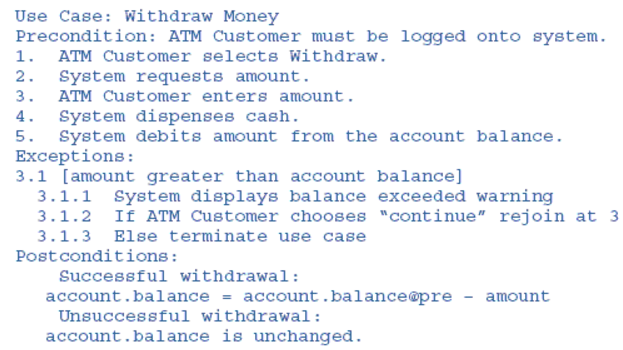
\includegraphics[width=0.8\textwidth]{images/Use_Case_Example}
\caption{Use case example. Source: \cite{Williams_et_dot_al_2005}.}
\label{fig:use_case_example}
\end{figure}

\subsection{Traditional Requirements Quality}

Requirements validation is a phase on traditional RE process that is known to support requirements elicitation, requirements analysis and requirements specification activities by identifying and correcting errors in the requirements \cite{Heikkila_et_dot_al_2015}. G{\'e}nova \cite{Genova_2013} states that quality indicators must not provide numerical evaluations only, but first of all they must point out concrete defects and provide suggestions for improvement, just like a spell and grammar checker can help to improve the quality of a text. For Davis \cite{Davis_1993}, a perfect software requirements specification is impossible as some qualities may be achieved only on the expense of others. The author also implies that one must be careful to recognize that although quality is attainable, perfection is not.

The Business Analyst Body of Knowledge (BABOK) \cite{Babok_2015} states that, while quality is ultimately determined by the needs of the stakeholders who will use the requirements or the designs, acceptable quality requirements exhibit many characteristics. BABOK's second edition \cite{Babok_2009} describes eight characteristics a requirement must have in order to be a quality one, as follows: adaptability, cohesion, completeness, consistency, correction, testability, unambiguity, and viability. BABOK's third edition \cite{Babok_2015} brings nine: atomic, complete, consistent, concise, feasible, prioritized, testable, unambiguous, and understandable. Both editions \cite{Babok_2009}\cite{Babok_2015} define what each characteristic means, but do not provide any measurement guidance.

Use cases quality is discussed in details by Phalp et. al \cite{Phalp_et_dot_al_2011}. Their study summarizes prior work on use cases quality (such as the rules found by Cockburn \cite{Cockburn_2000}) and proposes refined rules based on discourse process theory, such as avoiding the use of pronouns, use active voice over passive one, achieve simplicity trough avoiding to use negative forms, adjectives and adverbs, use of discourse cues, and the effect of readers background and goals. Also, desirable quality attributes of use cases are listed, that may be suited for certain project phases but not others as follows: standard format, completeness, conciseness, accuracy, logic, coherence, appropriate level of detail, consistent level of abstraction, readability, use of natural language, and embellishment. The authors create rules, that should be enforced and must be obeyed, and guidelines, which indicate an ideal that cannot always be followed, that could best produce those attributes. 

El-Attar and Miller \cite{Attar_2012} present another list of use cases qualities attributes - this time, applied to use case diagrams. The list contains the following attributes: consistency, correctness and completeness, fault-free, analytical, and understandability. Along with the attributes, the authors had performed a systematic literature review and identified 61 unique guidelines, heuristics and rules for these format of requirements, that were synthesized and compiled into a set of 21 anti-patterns, a literary form that describes a commonly occurring solution to a problem that generates decidedly negative consequences.

\subsection{Reviews and Inspections}

BABOK's 3rd edition \cite{Babok_2015} argues that one way to validate quality characteristics is through a review, as they can help identify defects early in the work product life cycle, eliminating the need for expensive removal of defects discovered later in the life cycle. 

Melo et. al \cite{Melo_et_dot_al_2001} state that software review activities can be applied at many points during the software development process and can be used to discover defects in any type of deliverables or internal work products. Thus, software review activities have the ``purification effect'' of software artifacts as an objective. Inspection, a form of review, is a rigorous defect detection process. The advantages of this inspection review process are: there is an effective mistake detection mechanism; qualitative and quantitative project feedback is given earlier; and a record of the inspection is kept, allowing the evaluation of the task performed \cite{Melo_et_dot_al_2001}. 

Laitenberger \cite{Laitenberger_2002} expects that inspection results depend on inspection participants themselves and their strategies for understanding the inspected artifact. Therefore, supporting inspection participants (inspectors) with particular techniques that help them detect defects in software products may increase the effectiveness of an inspection team. Such techniques are referred as reading techniques. 

Zhu \cite{Zhu_2016} describes software inspection as a formalized peer review process applicable to any software artifact. According to him, it is widely established that software inspection is effective (it finds many defects), efficient (low cost per defect), and practical (easy to carry out). The immediate benefit of software review is to detect and fix errors or problems in software artifacts, which become more readable and maintainable \cite{Zhu_2016}.

Zhu \cite{Zhu_2016} states that software review is primarily an individual effort and the kinds of reading techniques the individual uses are paramount to the outcome and effectiveness of software review. This thought is reinforced by Shull and colleagues \cite{Shull_et_dot_al_2003}, as these authors state that, while typical inspections require individuals to review a particular artifact to next meet as a team to discuss and record defects, empirical evidence has questioned the importance of team meetings by showing that meetings do not contribute to finding a significant number of new defects that were not already found by individual reviewers. 

\subsection{Reading Techniques}

A software reading technique is a series of steps for the individual analysis of a textual software product to achieve the understanding needed for a particular task - thus demonstrating that reading has a purpose and is an individual activity \cite{Zhu_2016} \cite{Shull_et_dot_al_2003}. For Melo et. al \cite{Melo_et_dot_al_2001}, those techniques attempt to capture knowledge about best practices for defect detection into a procedure that can be followed and also to achieve the understanding needed for a particular task. In a sense, a reading technique can be regarded as a mechanism or strategy for the individual inspector to detect defects in the inspected product \cite{Laitenberger_2002}.

Shull et. al \cite{Shull_et_dot_al_2003} declare that software reading techniques can be applied to improve the effectiveness of software inspections by improving the effectiveness of individual reviewers. Zhu \cite{Zhu_2016} further defines that a series of steps is a set of instructions that guide the reader how to read the artifacts, what areas to focus on and what problems to look for, while Shull et. al \cite{Shull_et_dot_al_2003} define them as two components: (a) a concrete procedure that can be followed to focus on only the information in the review document that is important for the quality aspects of interest, and (b) questions that explicitly ask the reader to think about the information just uncovered in order to find defects. For the purpose of our research, we use Shull et. al's definition \cite{Shull_et_dot_al_2003} to motivate the organization of our proposed question-based checklist.

The most widely used format of reading technique are checklists \cite{Zhu_2016}. Zhu defines it as a list of questions to provide reviewers with hints and recommendations for finding defects during the examination of software artifacts. Since a question can be rephrased as an imperative sentence, the checklist does not have to be composed of questions only - matching his flexible definition for reading techniques. One example of checklist is the questionnaire used by Cockburn \cite{Cockburn_2000} to evaluate the quality of Use Cases, shown in Figure \ref{fig:cockburn_usecase_questionnaire}. 

\begin{figure}
	\centering
	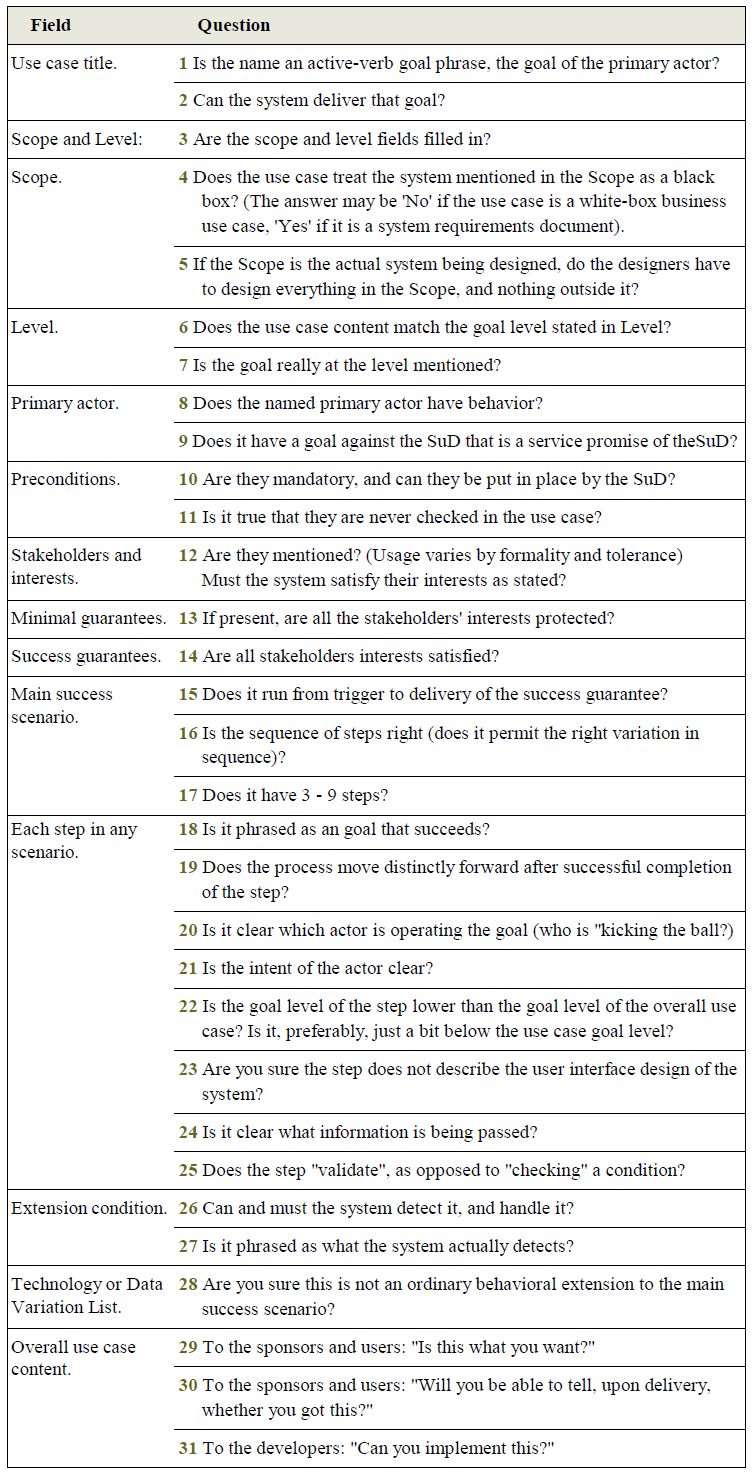
\includegraphics[scale=0.7]{images/cockburn_usecase_questionnaire}
	\caption{Cockburn's use case questionnaire. Source: \cite{Cockburn_2000}}
	\label{fig:cockburn_usecase_questionnaire}
\end{figure}

Laitenberger \cite{Laitenberger_2002} found that ad-hoc reading and checklist-based reading are the most popular reading techniques used today for defect detection during inspection. Ad-hoc reading offers very little reading support at all since a software product is simply given to inspectors without any direction or guidelines on how to proceed through it and what to look for. It does not, however, mean that inspection participants do not scrutinize the inspected product systematically. The word "ad-hoc" refers to the fact that no technique is used to support the reviewers on the problem of how to detect defects in a software artifact -- defect detection fully depends on the skill, the knowledge, and the experience of the reviewer. Training sessions may help subjects develop some of these capabilities to alleviate the lack of reading support.

Checklists offer stronger support in the form of questions. Although reading support in the form of a list of questions is better than none, Laitenberger \cite{Laitenberger_2002} considers several weaknesses on checklist-based reading, as follows: the questions are often general and not sufficiently tailored to a particular development environment; concrete instructions on how to use a checklist are often missing, that is, it is often unclear when and based on what information an inspector is to answer a particular checklist question; and questions are often limited to the detection of defects that are based on past defect information. 

For our purposes, we decided that having an instrument similar to Cockburn's checklist \cite{Cockburn_2000} in the form of question-based checklist to evaluate the quality of use cases is a reasonable first step to bring reading techniques to BDD scenarios.

\section{Agile Requirements}

Agile software development methods take a different approach to RE and communication than the traditional RE approaches that are mostly based on formal documents and defined phases \cite{Heikkila_et_dot_al_2015}. Through the mapping of a systematic literature reviews on the subject, Heikkila and colleagues \cite{Heikkila_et_dot_al_2015} have pointed out some benefits and challenges for RE on agile contexts. 

Two important challenges to note in the Heikkila and colleagues study \cite{Heikkila_et_dot_al_2015} are the insufficiency of the user story format and the reliance on tacit requirements knowledge. The first challenge comes from the fact that user stories do not convey enough information for software design and separate systems and subsystem are required to fill that hole. The second challenge is due to the fact that requirements knowledge is mostly tacit. Section \ref{chap:chap2_user_stories} will describe user stories to help on the understanding of those problems, while Section \ref{chap:chap2_acceptance_tests} will describe acceptance tests, a way to express requirements details that do not fit the user story model. 

The need to better describe those tests and how they bound together with user stories is reinforced by Bjarnason et. al \cite{Bjarnason_et_dot_al_2016}, who described how tests are used as requirements on agile contexts. One of the companies on their study uses a BDD approach, where requirements are documented upfront as automated acceptance test cases as part of the elicitation process and are expressed in a structured format in a way that the specification can be executable. This approach is explained in details in Section \ref{chap:chap2_bdd}.

\subsection{\label{chap:chap2_user_stories}User Stories}

Traditional RE activities have become too abstract and moved away from how people ordinarily learn and communicate - too far away from storytelling, something that everyone understands intuitively \cite{Rinzler_2009}. By using storytelling, the process of gathering information and structuring the requirements document would be immediately improved, as the author understands that one instinctively transform abstract knowledge into a logical structure when telling a story. 

Agile methodologies are sympathetic with this thought and represent requirements using user stories. This form of requirements representation have been created along with the Extreme Programming (XP) methodology, where each story describes one thing that the system needs to do as described by Jeffries et. al \cite{Jeffries_et_dot_al_2000}. They are written by a customer (or a customer team) to a development team, who have the responsibility to understand the story and design, build and test a software that implement it. User Stories bring together the rights of customers, who have the right to get the most possible value out of every programming moment, by asking for small atomic bits of functionality, and developers, who have the right to know what is needed. They are a short description of the behavior of the system from the point of view of the user of the system and are backed up with conversation and perhaps with some related detailed information. 

Furthermore, a user story represents a feature a customer wants in the software, a story she would like to be able to tell her friends about this great system she is using \cite{Beck_Fowler_2000}. A user story is a specific thing that would make the system easy to use, a chunk of functionality that is of value to the customer. As a unit of functionality, the team demonstrates progress by delivering tested, integrated code that implements a story. The customer must write the story in cards, and it  is up to the developers to estimate it trough collaboration with the customer.

For Cohn \cite{Cohn_2004}, a user story describes functionality that will be valuable to either a user or purchaser of a system or software. Each story must be written in the language of the business, not in technical jargon, so that the customer team can prioritize the stories for inclusion into iterations and releases. The author provides some reasons on why user stories are used, as follows: they emphasize verbal rather than written communication; are comprehensible by both the customer and the developers; and encourage deferring detail until the team, customers and developers, have the best understanding they are going to have about what they really need. While Jeffries et. al \cite{Jeffries_et_dot_al_2000} list only two aspects of user stories -- the short description of it and the conversations around it, Cohn \cite{Cohn_2004} composes a User Story using three aspects:

\begin{itemize}
    \item a written description of the story used for planning and as a reminder;
    \item conversations about the story that serve to flesh out the details of the story; and
    \item tests that convey and document details and that can be used to determine when a story is complete.
\end{itemize}

Those aspects have come from the Card, Conversation and Confirmation terms defined by Jeffries et. al \cite{Jeffries_2001}. Cohn described that the Card represents customer requirements rather than document them, has just enough text to identify the requirement, and to remind everyone what the story is. The Conversation is an exchange of thoughts, opinions, and feelings. It is largely verbal, but can be supplemented with documents. The best supplements are examples and the best examples should be executable. They are representations of the Confirmation, a way to customers tell developers how they will confirm that they have done what is needed in the form of acceptance tests. That confirmation, provided by those examples, is what makes possible the simple approach of card and conversation. When the conversation about a card gets down to the details of the acceptance test, the customer and programmer settle the final details of what needs to be done.

The main format of a user story, popularized by Cohn's book \cite{Cohn_2004}, is: I as a \textit{role} want \textit{function} so that \textit{business value}. Lucassen et. al \cite{Lucassen_et_dot_al_2015} summarize that user stories only capture the essential elements of a requirement: \textit{who} it is for, \textit{what} it expects from the system, and, optionally, \textit{why} it is important. As user stories express \textit{what} is desired and \textit{why} it is needed by the client, this requirement format is better compared to business or stakeholders requirements \cite{Babok_2009}\cite{Babok_2015}.

\subsection{\label{chap:chap2_acceptance_tests}Acceptance Tests}

Acceptance testing is the process of verifying that user stories were developed such that each works exactly the way the customer team, the ones who write user stories on XP methodology, expected it to work \cite{Cohn_2004}. Acceptance tests are specified as soon as the iteration begins and, depending on the customer team's technical expertise, can be put into an automated testing tool. Those tests help the customer team to communicate assumptions and expectations to the developers, by expressing the details that result from the conversations between customers and developers, and also by validating that a story has been developed with the functionality the team members had in mind when they wrote the story. New tests should be added as long as they add value and clarification to the story. Their scope should focus on clarifying the intent of the story to the developers instead of covering all the low level possible validations, like testing invalid dates range.

Jeffries et. al \cite{Jeffries_et_dot_al_2000} said that acceptance tests allow the customer to know when the system works, and tell the programmers what needs to be done. In the XP methodology, programmers have the right to know what is needed and customers have the right to see progress in a running system, proven to work by specified automated test. These tests provide confidence that the system really does what it needs to do.

For Beck and Fowler \cite{Beck_Fowler_2000}, acceptance tests execution will determine whether the user stories have been successfully implemented. Also, once acceptance tests are running, the story card can be discarded, since they are encoded in far more detail and accuracy in the acceptance tests, so no information will be lost if the cards are destroyed.

Gartner \cite{Gartner_2012} reported that the hardest job in software development is communicating clearly about what one wants the system to do. Guiding the development effort with acceptance tests helps with this challenge. Two core practices are described in his book to address such a challenge, as follows: (a) before implementing each feature, team members collaborate to create concrete examples of the feature in action and (b) then the team translates these examples into automated acceptance tests, that become a prominent part of the team's shared and precise description of ``done'' for each feature. Teams that follow those practices are working on the Acceptance Test-Driven Development (ATDD) way.

Haugset and Stalhane \cite{Haugset_2012} describe ATDD as a mixture of the traditional documentation-centric RE and the communication-focused iterative agile RE, carrying its own set of benefits and challenges. The benefits stem both from the inherent strengths that lie in discussing requirements using the acceptance tests as a mediator and its abilities for automation of the same tests. On the case study described by the authors, the ATDD technique was used to help communicate requirements (externalization) in the specification phase, helping to uncover, understand and describe requirements. In the study's verification phase, ATDD was used to automatically verify that the code adhered to the customer requirement on an acceptance level, accompanied by manual testing for certain issues. The authors judge that ATDD saves effort in the long run, despite having a higher upfront cost due to the need of even more interaction with customers than agile development does, since the tests act as a safety harness for making changes and acts as documentation of code.

In short, as acceptance tests describe the expectations that a system must show in order to demonstrate that the application is acceptable by the customer \cite{Cohn_2004} and can fill the documentation role of functional requirements \cite{Babok_2009}\cite{Babok_2015}. Yet, due to the fact that they are often automated test and often written by customers with their own words, they can also fill the living documentation vision proposed by Adzic's Specification by Example book \cite{Adzic_2011}.

\subsection{\label{chap:chap2_bdd}Behavior-Driven Development}

One way to represent acceptance tests are scenarios. Alexander and Maiden \cite{Alexander_and_Maiden_2004} describe that the activity of building requirements scenarios encourages imagination and exploration while setting the stage for discovering unconscious and undreamed requirements. That is important because stories are the primary (perhaps only) means of communicating needs and desires, and providing critical feedback to developers.

Kaner \cite{Kaner_2003} describes scenarios as a hypothetical story used to help a person think through a complex problem or system. Scenarios also help in the product learning, as people do not learn well by following checklists or material that is organized for them -- people often learn by doing tasks that require them to investigate the product for themselves. The author also brings the idea that a scenario is an instantiation of a use case—take a specific path through the model, assigning specific values to each variable. Finally, as the scenario is a story about someone trying to accomplish something with the product under test, it can help to expose failures to deliver desired benefits.

Scenarios can also represent the key examples that describe the expected functionality, a concept introduced by Adzic \cite{Adzic_2011}. The living documentation presented by the author helps to validate if the system works in the same way reflected by the documentation that represents it. Example tables are also used on the mentioned book, where one represents the system's inputs and outputs using tables where each row represents a given example. Specialized tools, like the framework for integrated tests shown by Gartner \cite{Gartner_2012}, can read those tables and use them on the software under test. 

%bdd introduction
Behavior-Driven Development (BDD) is a set of practices that uses scenarios as an business-readable language to describe and model a system \cite{Smart_2014}. Scenarios are expressed in a format known as Gherkin, that is designed to be both easily understandable for business stakeholders and easy to automate using dedicated tools. According to the author, bringing business and technical parties together to talk about the same document helps to build the right software (the one that meets customer needs) and to build it right (without buggy code). Those scenarios are referred as structured examples, in a similar way as Adzic \cite{Adzic_2011} calls them key examples. Many ideas are similar on both publications. As explained by Smart \cite{Smart_2014}, using conversation and examples to specify how one expects a system to behave is a core part of BDD. 

This idea of using conversation and examples to specify a system behavior is reinforced by Wynne and Hellesoy \cite{Wynne_and_Hellesoy_2012} discourse on their book about Cucumber, a library that implements BDD scenarios for the Ruby programming language. The authors state that software teams work best when the developers and business stakeholders are communicating clearly with one another -- and a great way to do that is to collaboratively specify the work that is about to be done using automated acceptance tests. Additionally, when the acceptance tests are written as examples, they stimulate people’s imaginations and help them see other scenarios they had not previously considered. Most important is the fact that, when the team members write their acceptance tests collaboratively, they can develop their own ubiquitous language to talk about their problem domain -- a common language that helps them avoid misunderstandings.

% bdd == acceptance tests
BDD practitioners collaborate with the user to find concrete examples to illustrate features requested to the development team. Quite often, they also automate the execution of those scenarios. Since they are written to express the details and help the customer accept a given feature, they can be used as acceptance tests. Also, the collaboration among development team and customers that is needed to write those scenarios can be mapped as the conversations about a story that Cohn \cite{Cohn_2004} and Jeffries \cite{Jeffries_2001} mentioned.

In Gherkin, the scenarios related to a particular feature are grouped into a single text file called a feature file. A feature file contains a short description of the feature, followed by a number of scenarios, or formalized examples of how a feature works. Each scenario is made up of a number of steps, where each step starts with one of a small set of keywords: \textit{Given} describes the preconditions for the scenario and prepares the test environment; \textit{When} describes the action under test; \textit{Then} describes the expected outcomes. One example of a scenario for a train management application that should have a feature to help a commuter to find the optimal itinerary between stations on the same line defined by Smart \cite{Smart_2014} is presented in Figure \ref{fig:scenario_example}.

\begin{figure}[t]
\centering
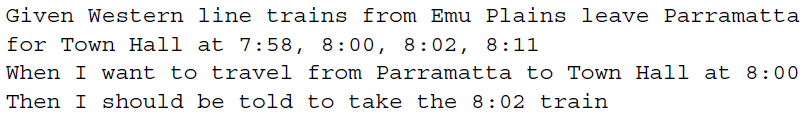
\includegraphics[scale=0.7]{images/smart_scenario_example}
\caption[Scenario example]{Scenario example. Source \cite{Smart_2014}.}
\label{fig:scenario_example}
\end{figure}

\begin{figure}[t]
\centering
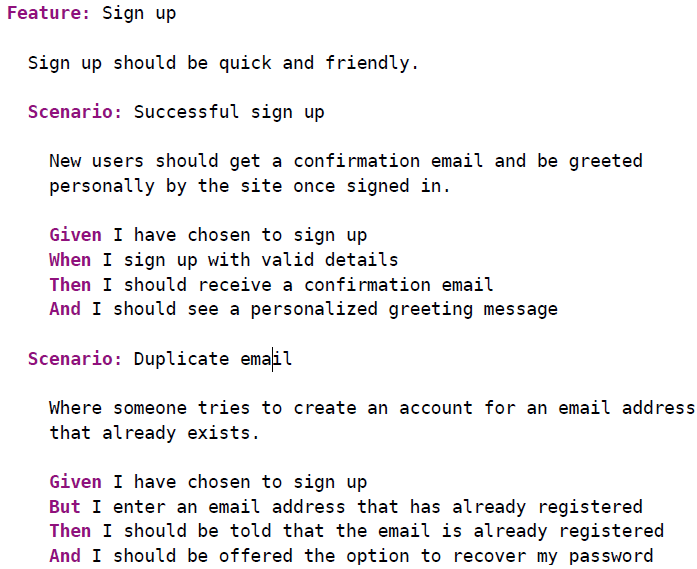
\includegraphics[scale=0.7]{images/feature_file_example}
\caption[Feature file example]{Feature file example. Source \cite{Wynne_and_Hellesoy_2012}}
\label{fig:feature_file}
\end{figure}

Multiple scenarios can be grouped together into feature files, such as the one in Figure \ref{fig:feature_file} which groups together two scenarios related to sign-in feature -- the first represents a successful login, while the second represents a duplicate e-mail situation. Each of those scenarios has a title and a short description before the steps are described. Also, the beginning of the feature file has a description of the feature being tested by those scenarios.

Along with the features, one should provide to specialized tools, such as Cucumber, a set of step definitions, which
map the business-readable language of each step into a code written in a certain programming language to carry out whatever action is being described by the step. This hierarchy, from features down to automation library, is illustrated in Figure \ref{fig:bdd_stack}. In this thesis, we are only concerned with the business facing aspects of a BDD scenario, represented by the feature, the scenario and the step boxes in Figure \ref{fig:bdd_stack}.

\begin{figure}[t]
\centering
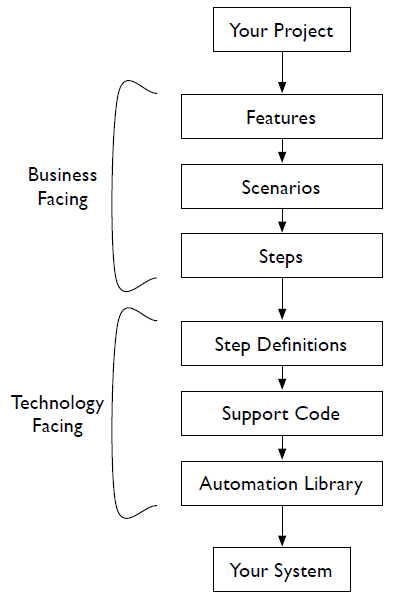
\includegraphics[scale=0.7]{images/bdd_stack}
\caption{Typical stack of a BDD tool such as Cucumber. Source \cite{Wynne_and_Hellesoy_2012}}
\label{fig:bdd_stack}
\end{figure}

Regarding the process used to specify those scenarios, Smart \cite{Ferguson_2017} describes each stage of a feature worked by a team following a BDD process, as shown in Figure \ref{fig:bdd_process}, as a set of cyclical stages, described as follows: 

\begin{figure}
\centering
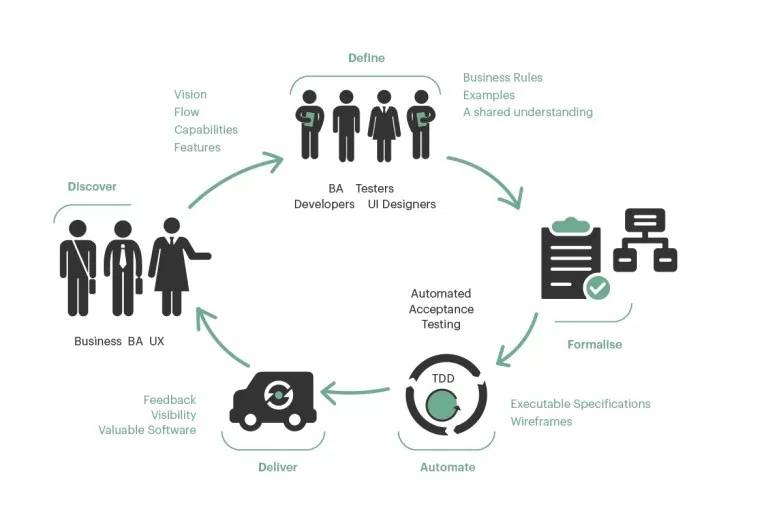
\includegraphics[scale=0.6]{images/bdd}
\caption{Typical stages of a feature on a BDD process. Source \cite{Ferguson_2017}}
\label{fig:bdd_process}
\end{figure}

\begin{itemize}
    \item \textbf{Discover stage}: during this early stage, high level techniques, like Story Mapping \cite{Paton_User_Story_Mapping_2014} and Impact Mapping \cite{Gojko_Impact_Mapping_2012}, can help get an overall picture of what one is trying to achieve \cite{Ferguson_2017}. Additionally, Smart \cite{Ferguson_2017} points out that \textit{at this stage, the emphasis is on breadth, rather than detail};
    
    \item \textbf{Define stage:} in this stage the team starts to have more concrete conversations around more specific business rules and examples of how the user would interact with the system. Often referred simply as ``conversations'', in this stage the team should not get bogged down in the Gherkin syntax.
    
    \item \textbf{Formalize stage}: Smart \cite{Ferguson_2017} states that, once key business rules and examples have been identified they can be formalized into Gherkin by an engineer in test, often pairing with a Business Analyst or manual tester. Additionally, once they are ready, the Gherkin scenarios should be shared and discussed with the broader team, highlighting the need to acquire team's feedback on scenarios, a common behavior we saw on many participants. This is the stage where our research is focused on, as we seek to provide a quality evaluation instrument to aid in the assessment of scenario's quality;
    
    \textbf{Automate and Deliver stages}: this is the stage where the team will create the missing piece of functionality and these Gherkin scenarios will be automated. It is outside of this thesis scope to evaluate the source code that transforms each Gherkin step into an executable script.

\end{itemize}

% bdd == use cases == functional requirements.
BDD scenarios are similar to use cases scenarios as they both describe a system behavior under certain precondition (expressed on the \textit{Given} clauses of a BDD scenario) to achieve a certain goal (expressed on the \textit{Then} clauses of a BDD scenario). As they are a format to express acceptance tests, described in Section \ref{chap:chap2_acceptance_tests}, they can also fill the documentation role of functional requirements \cite{Babok_2009}\cite{Babok_2015}. Finally, due to the fact that they are often automated test and are written on a ubiquitous language that should be understood by everyone in the project, they can also fill the living documentation vision proposed by Adzic \cite{Adzic_2011}.

\subsection{\label{chap:chap2_agile_quality}Agile Requirements Quality}

Lucassen et. al \cite{Lucassen_et_dot_al_2015} report that the number of methods to assess and improve user story quality is limited. Existing approaches to user story quality employ highly qualitative metrics, such as the heuristics of the INVEST (Independent-Negotiable-Valuable-Estimable-Scalable-Testable) framework described by Cohn \cite{Cohn_2004}. Due to that fact, Lucassen et. al \cite{Lucassen_et_dot_al_2015} define additional criteria to evaluate user stories on their QUS Framework, as follows: atomic, minimal, well-formed, conflict-free, conceptually sound, problem-oriented, unambiguous, complete, explicit dependencies, full sentence, independent, scalable, uniform, and unique.

For acceptance tests, our understanding is that this kind of tests should meet the quality attributes that all requirements from both BABOK versions \cite{Babok_2009}\cite{Babok_2015} meet, as we compare acceptance tests with functional requirements, and the ones for use cases found by Cohn \cite{Cockburn_2000} and Phalp et. al \cite{Phalp_et_dot_al_2011}. However, little work has been found to support this understanding. 

%generic scenarios characteristics
Generic scenarios quality evaluation seems to be based upon subjective characteristics, like the ones found by Kaner \cite{Kaner_2003}, or on generic guidelines, like what Alexander and Maiden \cite{Alexander_and_Maiden_2004} had highlighted. Kaner \cite{Kaner_2003} describes that a test based in a scenario has five characteristics, as follows: it is (a) a story that is (b) motivating, (c) credible, (d) complex, and (e) easy to evaluate. Nevertheless, empirical evaluation of existing acceptance test cases expressed as scenarios according to his characteristics were not found. Alexander and Maiden \cite{Alexander_and_Maiden_2004} define a guideline that should be used for use cases and scenarios alike - their view seems to indicate that acceptance tests fill the same role on requirements documentation.  

To the best of our knowledge, BDD scenarios are only being evaluated based on characteristics, such as those taken from Smart \cite{Smart_2014} and Wynne and Hellesoy \cite{Wynne_and_Hellesoy_2012} experiences: scenarios steps expressiveness; focus the steps on what goal the user want to accomplish and not on implementation details or on screen interactions (writing it in a declarative way and not on a imperative way); the use of preconditions on the past tense, to make it transparent that those are actions that have already occurred in order to begin that test; the reuse of information to avoid unnecessary repetition of words; and the scenarios independence. Even though the authors \cite{Smart_2014}\cite{Wynne_and_Hellesoy_2012} specify a few scenarios as examples to demonstrate those described characteristics, we feel that BDD scenarios could benefit from a question-based checklist defined from the collective knowledge of other practitioners, similar to the one defined by Cockburn for use cases \cite{Cockburn_2000}.

\section{Conclusion}

The quality characteristics shown on both versions of the BABOK \cite{Babok_2009}\cite{Babok_2015} have taught us that traditional requirements writers have many guides to help them evaluate their work like the ones described by Laitenberger \cite{Laitenberger_2002} and Melo et. al \cite{Melo_et_dot_al_2001}. Also, Phalp et. al \cite{Phalp_et_dot_al_2011} have shown that use cases quality criteria and guidelines are also mature enough to help practitioners writing them. Finally, user stories writers have informal guidelines (such as the INVEST acronym used by Cohn \cite{Cohn_2004}) and an ongoing study on quality characteristics (from Lucassen et. al \cite{Lucassen_et_dot_al_2015}) to help on their efforts. On the other hand, the quality of acceptance tests is still open to debate, with only a few characteristics (found by Kaner \cite{Kaner_2003}, Smart \cite{Smart_2014} and Wynne and Hellesoy \cite{Wynne_and_Hellesoy_2012}) or generic guidelines (like the one created by Alexander and Maiden \cite{Alexander_and_Maiden_2004}) to use, all without empirical evaluation to certify their usefulness. No reading technique were found to address acceptance tests as well.  

On agile contexts, requirements are represented mainly as user stories according to Lucassen et. al \cite{Lucassen_et_dot_al_2015}. Due to that fact, it makes sense that the authors focus their quality framework on the user story card representation from Cohn \cite{Cohn_2004} only, letting the details that are expressed as acceptance tests out of it. However, due to the growing importance of requirements expressed as tests shown by Bjarnason et. al \cite{Bjarnason_et_dot_al_2016}, we believe this gap needs to be filled.

BDD is a format to represent acceptance tests, as stated by Gartner \cite{Gartner_2012}, that was used on one of the companies interviewed by Bjarnason et. al \cite{Bjarnason_et_dot_al_2016} study and to which only informal characteristics exists to evaluate them, either from Smart's experiences \cite{Smart_2014} or Wynne and Hellesoy's \cite{Wynne_and_Hellesoy_2012}. Since BDD scenarios represent the intended behavior of a system, the quality attributes for use cases and functional requirements could be re-used -- but no study was found on that area. Also, the framework from Lucassen et. al \cite{Lucassen_et_dot_al_2015} could be expanded to also cover BDD scenarios -- but again, no efforts on that direction have been found. Finally, having a set of attributes to evaluate a written work without a strategy or a way to use them properly may not be enough to help a writer be more effective. Thus, there is also the need to provide a way to guide the software development team members on how to proper use those attributes in a review process.
